\begin{appendices}
    \newpage
    \section{Codificación Entradas-Salidas} \label{app:codEntSal}
    
        \begin{table}[H]
        \centering
			\begin{tabular}{|c|c|c|c|}
				\hline
				\rowcolor[rgb]{0.21,0.69,0.87}\multicolumn{4}{|c|}{  \textbf{ {Codificación Pisos}}} \\
				\hline \hline
				 & \textbf{  PisoVoy (pulsadores)  } & \textbf{  PisoEstoy (finalCarrera)  } & \textbf{  7 Segmentos  }  \\
				\hline
				Piso1 & 0001 & 0001 & Imagen \\
				\hline
				Piso2 & 0010 & 0010 & Imagen \\
				\hline
				Piso3 & 0100 & 0100 & Imagen \\
				\hline
				Piso4 & 1000 & 1000 & Imagen \\
				\hline
				 
			\end{tabular}
			\caption{ Codificación para los diferentes pisos y su traducción  al número de piso y al display de 7 segmentos }
			\label{tab:tabla1ApendiceA}
		\end{table}
		
		
        \begin{table}[H]
        \centering
			\begin{tabular}{|c|c|}
				\hline
				\rowcolor[rgb]{0.21,0.69,0.87}\multicolumn{2}{|c|}{  \textbf{ {Funcionamiento Motor}}} \\
				\hline \hline
				 & \textbf{ Codificación Interna }  \\
				\hline
				Motor Parado & 00  \\
				\hline
				Motor girando en sentido de Subida & 01  \\
				\hline
				Motor girando en sentido de Bajada & 10 \\ 
				\hline
				 
			\end{tabular}
			\caption{ Codificación para los diferentes pisos y su traducción  al número de piso y al display de 7 segmentos }
			\label{tab:tabla2ApendiceA}
		\end{table}

		
	\section{Codificación para display de 7 segmentos}	\label{app:7segmentos}
		\begin{table}[H]
        \centering
			\begin{tabular}{|ccccc|}
				\hline
				\rowcolor[rgb]{0.21,0.69,0.87}\multicolumn{5}{|c|}{  \textbf{ {Caracteres en binario para display de 7 segmentos}}} \\
				\hline \hline
				\multicolumn{3}{|c|}{  \textbf{ {Funcionamiento Motor}}} & \multicolumn{2}{|c|}{\textbf{Funcionamiento Puerta}} \\
				\hline
				 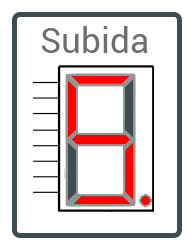
\includegraphics[width = 0.15\textwidth ]{CodCaracteres7s/subida} &
				 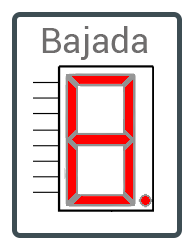
\includegraphics[width = 0.15\textwidth ]{CodCaracteres7s/bajada}  &
				 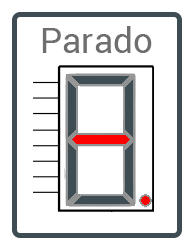
\includegraphics[width = 0.15\textwidth ]{CodCaracteres7s/parado} &
				 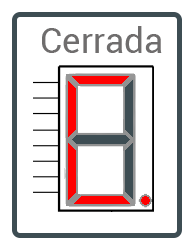
\includegraphics[width = 0.15\textwidth ]{CodCaracteres7s/Cerrada}  &
				 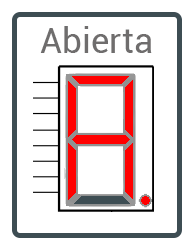
\includegraphics[width = 0.15\textwidth ]{CodCaracteres7s/abierta}  \\
				 1011011 & 1111111 & 0000001 & 1001110 & 1110111 \\ 	
				\hline
				 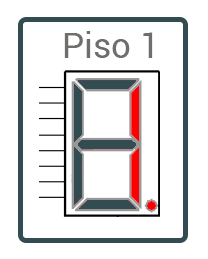
\includegraphics[width = 0.15\textwidth ]{CodCaracteres7s/p1} &
				 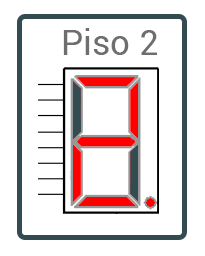
\includegraphics[width = 0.15\textwidth ]{CodCaracteres7s/p2}  &
				 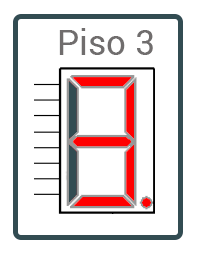
\includegraphics[width = 0.15\textwidth ]{CodCaracteres7s/p3} &
				 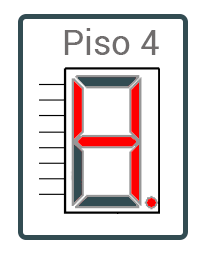
\includegraphics[width = 0.15\textwidth ]{CodCaracteres7s/p4}  &
				 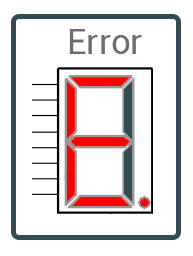
\includegraphics[width = 0.15\textwidth ]{CodCaracteres7s/error}  \\
				 1001111 & 0010010 & 0000110 & 1001100 & 0110000 \\ 
				\hline
			\end{tabular}
			\caption{ Codificación en binario para mostrar la información en el display de 7 segmentos }
			\label{tab:tabla1ApendiceB}
		\end{table}
	\newpage	
\end{appendices}